\section{Metric axioms. Metric spaces. Norms. Normed linear spaces}
\vspace*{-0.5cm}

\begin{definition}{(Metric space)}{}
    A metric space is a set $X$ with a metric $\rho: \ X \times X \to [0, \infty)$ (or it can be valid notation $d$, in that way we can call it by `distance') such that $\forall x, y, z \in X$, $\rho$ satisfies the following properties:
    \begin{enumerate*}
        \item Positive definite:
        \[
            \begin{array}{c}
                \rho(x,y) \geq 0, \ \ \forall x \neq y\\
                \rho(x,y)=0\Longleftrightarrow x = y; \ \rho(x,x) = 0.
            \end{array}  
        \]
        \item Symmetric:
        \[
            \rho(x,y) = \rho(y,x).  
        \]
        \item Triangle Inequality:
        \[
            \rho(x, z) \leq \rho (x,y) + \rho(y,z).  
        \]
    \end{enumerate*}
\end{definition}
\Ex

\begin{wrapfigure}[10]{l}{0.5\columnwidth}
    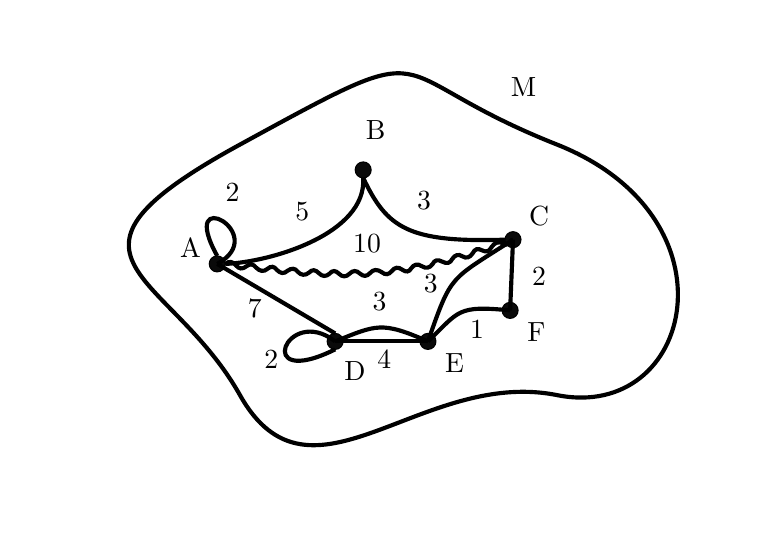
\begin{tikzpicture}[x=0.75pt,y=0.75pt,yscale=-1,xscale=1]
        %uncomment if require: \path (0,300); %set diagram left start at 0, and has height of 300
        
        %Shape: Regular Polygon [id:dp5338509974760937] 
        \draw  [line width=1.5]  (120,78.65) .. controls (221.27,23.33) and (183.93,43.45) .. (272.76,78.65) .. controls (361.58,113.86) and (338.39,212.43) .. (272.76,199.36) .. controls (207.13,186.28) and (153.94,259.71) .. (120,199.36) .. controls (86.05,139.01) and (18.72,133.98) .. (120,78.65) -- cycle ;
        %Shape: Ellipse [id:dp9070832079007569] 
        \draw  [fill={rgb, 255:red, 0; green, 0; blue, 0 }  ,fill opacity=0.96 ] (105.2,136.14) .. controls (105.2,134.02) and (106.92,132.29) .. (109.04,132.29) .. controls (111.17,132.29) and (112.89,134.02) .. (112.89,136.14) .. controls (112.89,138.27) and (111.17,139.99) .. (109.04,139.99) .. controls (106.92,139.99) and (105.2,138.27) .. (105.2,136.14) -- cycle ;
        %Shape: Ellipse [id:dp5742750162014552] 
        \draw  [fill={rgb, 255:red, 0; green, 0; blue, 0 }  ,fill opacity=0.96 ] (175.53,90.87) .. controls (175.53,88.74) and (177.25,87.02) .. (179.37,87.02) .. controls (181.49,87.02) and (183.21,88.74) .. (183.21,90.87) .. controls (183.21,93) and (181.49,94.72) .. (179.37,94.72) .. controls (177.25,94.72) and (175.53,93) .. (175.53,90.87) -- cycle ;
        %Shape: Ellipse [id:dp36112517430078106] 
        \draw  [fill={rgb, 255:red, 0; green, 0; blue, 0 }  ,fill opacity=0.96 ] (247.71,124.47) .. controls (247.71,122.35) and (249.43,120.62) .. (251.56,120.62) .. controls (253.68,120.62) and (255.4,122.35) .. (255.4,124.47) .. controls (255.4,126.6) and (253.68,128.32) .. (251.56,128.32) .. controls (249.43,128.32) and (247.71,126.6) .. (247.71,124.47) -- cycle ;
        %Shape: Ellipse [id:dp07609609258594396] 
        \draw  [fill={rgb, 255:red, 0; green, 0; blue, 0 }  ,fill opacity=0.96 ] (246.32,158.55) .. controls (246.32,156.42) and (248.04,154.7) .. (250.16,154.7) .. controls (252.28,154.7) and (254,156.42) .. (254,158.55) .. controls (254,160.67) and (252.28,162.4) .. (250.16,162.4) .. controls (248.04,162.4) and (246.32,160.67) .. (246.32,158.55) -- cycle ;
        %Shape: Ellipse [id:dp6798590078293778] 
        \draw  [fill={rgb, 255:red, 0; green, 0; blue, 0 }  ,fill opacity=0.96 ] (206.73,173.48) .. controls (206.73,171.35) and (208.45,169.63) .. (210.57,169.63) .. controls (212.69,169.63) and (214.41,171.35) .. (214.41,173.48) .. controls (214.41,175.61) and (212.69,177.33) .. (210.57,177.33) .. controls (208.45,177.33) and (206.73,175.61) .. (206.73,173.48) -- cycle ;
        %Shape: Ellipse [id:dp7303084540397591] 
        \draw  [fill={rgb, 255:red, 0; green, 0; blue, 0 }  ,fill opacity=0.96 ] (162.02,173.48) .. controls (162.02,171.35) and (163.74,169.63) .. (165.86,169.63) .. controls (167.98,169.63) and (169.7,171.35) .. (169.7,173.48) .. controls (169.7,175.61) and (167.98,177.33) .. (165.86,177.33) .. controls (163.74,177.33) and (162.02,175.61) .. (162.02,173.48) -- cycle ;
        %Curve Lines [id:da6929572494700036] 
        \draw [line width=1.5]    (179.37,94.72) .. controls (190.78,118.64) and (200.67,125.99) .. (247.71,124.47) ;
        %Curve Lines [id:da578214992025613] 
        \draw [line width=1.5]    (112.89,136.14) .. controls (134.54,135.33) and (181.11,121.79) .. (179.37,94.72) ;
        %Curve Lines [id:da3039206255102158] 
        \draw [line width=1.5]    (109.04,132.29) .. controls (89.37,96.74) and (135.47,121.63) .. (109.04,136.14) ;
        %Curve Lines [id:da9967226645293215] 
        \draw [line width=1.5]    (165.86,177.33) .. controls (125.69,197.25) and (142.46,155.24) .. (165.86,173.48) ;
        %Curve Lines [id:da770802220550038] 
        \draw [line width=1.5]    (112.89,136.14) .. controls (114.82,134.7) and (116.53,134.91) .. (118.02,136.78) .. controls (119.49,138.64) and (121.14,138.84) .. (122.99,137.38) .. controls (124.8,135.91) and (126.4,136.1) .. (127.8,137.94) .. controls (129.7,139.83) and (131.51,140.03) .. (133.23,138.54) .. controls (134.92,137.05) and (136.42,137.2) .. (137.74,139.01) .. controls (139.55,140.86) and (141.25,141.03) .. (142.85,139.5) .. controls (144.9,138.01) and (146.55,138.15) .. (147.81,139.92) .. controls (149.54,141.73) and (151.37,141.86) .. (153.31,140.32) .. controls (154.76,138.74) and (156.32,138.83) .. (158,140.59) .. controls (159.69,142.33) and (161.43,142.4) .. (163.23,140.79) .. controls (164.56,139.16) and (166.05,139.19) .. (167.72,140.89) .. controls (169.41,142.56) and (171.09,142.56) .. (172.77,140.89) .. controls (174.4,139.19) and (176.06,139.15) .. (177.75,140.77) .. controls (179.48,142.36) and (181.13,142.28) .. (182.7,140.53) .. controls (184.21,138.76) and (186.06,138.61) .. (188.24,140.1) .. controls (190.06,141.59) and (191.7,141.42) .. (193.17,139.58) .. controls (194.6,137.71) and (196.26,137.49) .. (198.14,138.91) .. controls (200.07,140.3) and (201.54,140.06) .. (202.54,138.21) .. controls (203.93,136.27) and (205.62,135.95) .. (207.63,137.26) .. controls (209.7,138.54) and (211.43,138.17) .. (212.83,136.16) .. controls (213.77,134.23) and (215.32,133.87) .. (217.48,135.06) .. controls (219.7,136.22) and (221.29,135.81) .. (222.24,133.83) .. controls (223.64,131.72) and (225.27,131.27) .. (227.13,132.48) .. controls (229.03,133.66) and (230.71,133.16) .. (232.16,130.98) .. controls (233.13,128.93) and (234.61,128.47) .. (236.6,129.59) .. controls (238.63,130.68) and (240.16,130.18) .. (241.17,128.09) .. controls (242.71,125.81) and (244.55,125.18) .. (246.68,126.21) .. controls (248.31,127.4) and (249.66,126.92) .. (250.73,124.77) -- (251.56,124.47) ;
        %Straight Lines [id:da9787751139512872] 
        \draw [line width=1.5]    (109.04,136.14) -- (165.86,169.63) ;
        %Straight Lines [id:da04164050721717438] 
        \draw [line width=1.5]    (251.56,124.47) -- (250.16,158.55) ;
        %Curve Lines [id:da9354219425220802] 
        \draw [line width=1.5]    (210.57,173.48) .. controls (222.1,140.62) and (220.7,144.35) .. (251.56,124.47) ;
        %Curve Lines [id:da9439539925566016] 
        \draw [line width=1.5]    (210.57,173.48) .. controls (225.82,158.82) and (224.43,156.02) .. (250.16,158.55) ;
        %Straight Lines [id:da35164383837720004] 
        \draw [line width=1.5]    (165.86,173.48) -- (210.57,173.48) ;
        %Curve Lines [id:da8246481493200473] 
        \draw [line width=1.5]    (165.86,173.48) .. controls (185.77,165.51) and (188.1,163.64) .. (210.57,173.48) ;
        
        % Text Node
        \draw (89.96,122.69) node [anchor=north west][inner sep=0.75pt]   [align=left] {A};
        % Text Node
        \draw (179.37,65.75) node [anchor=north west][inner sep=0.75pt]   [align=left] {B};
        % Text Node
        \draw (258.08,107.29) node [anchor=north west][inner sep=0.75pt]   [align=left] {C};
        % Text Node
        \draw (169.01,181.97) node [anchor=north west][inner sep=0.75pt]   [align=left] {D};
        % Text Node
        \draw (217.56,178.12) node [anchor=north west][inner sep=0.75pt]   [align=left] {E};
        % Text Node
        \draw (257.15,163.18) node [anchor=north west][inner sep=0.75pt]   [align=left] {F};
        % Text Node
        \draw (111.84,96.17) node [anchor=north west][inner sep=0.75pt]   [align=left] {$\displaystyle 2$};
        % Text Node
        \draw (145.38,105.5) node [anchor=north west][inner sep=0.75pt]   [align=left] {$\displaystyle 5$};
        % Text Node
        \draw (204.06,99.9) node [anchor=north west][inner sep=0.75pt]   [align=left] {$\displaystyle 3$};
        % Text Node
        \draw (259.48,136.77) node [anchor=north west][inner sep=0.75pt]   [align=left] {$\displaystyle 2$};
        % Text Node
        \draw (229.67,162.44) node [anchor=north west][inner sep=0.75pt]   [align=left] {$\displaystyle 1$};
        % Text Node
        \draw (207.32,140.04) node [anchor=north west][inner sep=0.75pt]   [align=left] {$\displaystyle 3$};
        % Text Node
        \draw (130.47,176.91) node [anchor=north west][inner sep=0.75pt]   [align=left] {$\displaystyle 2$};
        % Text Node
        \draw (122.56,152.17) node [anchor=north west][inner sep=0.75pt]   [align=left] {$\displaystyle 7$};
        % Text Node
        \draw (182.63,148.91) node [anchor=north west][inner sep=0.75pt]   [align=left] {$\displaystyle 3$};
        % Text Node
        \draw (184.96,176.91) node [anchor=north west][inner sep=0.75pt]   [align=left] {$\displaystyle 4$};
        % Text Node
        \draw (249.23,45.14) node [anchor=north west][inner sep=0.75pt]   [align=left] {M};
        % Text Node
        \draw (173.31,120.67) node [anchor=north west][inner sep=0.75pt]   [align=left] {$\displaystyle 10$};
        \end{tikzpicture}        
\end{wrapfigure}  

Let define some metric space with metric $\rho(x,y)$ is equal to the legth if the shortest path. Then $\dim (M) = 10$ and, e.g.:
\[
    \begin{array}{c}
        \rho(A,A) = 0;\\
        \rho(A, D) = 7;\\
        \rho(A, C) = 8
    \end{array}  
\]
Also we can show, for example, open ball on this example (we will define it little bit later):
\[
    \begin{array}{c}
        B_3(A) = \left\{A\right\}\\
        B_9(A) = \left\{A, B, C, D, E\right\}
    \end{array}  
\]

\par 
\Ex Given a set $X$:
\begin{itemize}
    \item The discrete metric $\rho$ on $X$ is defined by:
    \[
        \rho(x,y) = \left\{
            \begin{array}{cc}
                1 ,  & x \neq y\\
                0, & x = y.
            \end{array}
        \right.  
    \]
    \item Metric on continuous functions:
    \par 
    Let $X = \mathcal{C}[0,1] = \left\{\text{continuous functions } f: [0,1] \to \R\right\}$.
    Then we can define metrics:
    \[
            \begin{array}{c}
                \displaystyle\rho_0 (f,g) = \max\limits_{x \in [0,1]} |f(x) - g(x)|.\\
                \displaystyle\rho_1 (f,g) = \int\limits_{0}^1 |f(x) - g(x)|dx
            \end{array}
    \]
    Or: 
    \[
        \rho(f,g) = \rho_0(f,g) + |f(1) - g(1)|.
    \]
    \vspace*{-2cm}

    \begin{figure}[H]
        \centering

% Pattern Info
 


% Pattern Info
 
\tikzset{
pattern size/.store in=\mcSize, 
pattern size = 5pt,
pattern thickness/.store in=\mcThickness, 
pattern thickness = 0.3pt,
pattern radius/.store in=\mcRadius, 
pattern radius = 1pt}
\makeatletter
\pgfutil@ifundefined{pgf@pattern@name@_hx3fdizyv}{
\pgfdeclarepatternformonly[\mcThickness,\mcSize]{_hx3fdizyv}
{\pgfqpoint{0pt}{0pt}}
{\pgfpoint{\mcSize+\mcThickness}{\mcSize+\mcThickness}}
{\pgfpoint{\mcSize}{\mcSize}}
{
\pgfsetcolor{\tikz@pattern@color}
\pgfsetlinewidth{\mcThickness}
\pgfpathmoveto{\pgfqpoint{0pt}{0pt}}
\pgfpathlineto{\pgfpoint{\mcSize+\mcThickness}{\mcSize+\mcThickness}}
\pgfusepath{stroke}
}}
\makeatother

% Pattern Info
 
\tikzset{
pattern size/.store in=\mcSize, 
pattern size = 5pt,
pattern thickness/.store in=\mcThickness, 
pattern thickness = 0.3pt,
pattern radius/.store in=\mcRadius, 
pattern radius = 1pt}
\makeatletter
\pgfutil@ifundefined{pgf@pattern@name@_bfz0rqejm}{
\pgfdeclarepatternformonly[\mcThickness,\mcSize]{_bfz0rqejm}
{\pgfqpoint{0pt}{0pt}}
{\pgfpoint{\mcSize+\mcThickness}{\mcSize+\mcThickness}}
{\pgfpoint{\mcSize}{\mcSize}}
{
\pgfsetcolor{\tikz@pattern@color}
\pgfsetlinewidth{\mcThickness}
\pgfpathmoveto{\pgfqpoint{0pt}{0pt}}
\pgfpathlineto{\pgfpoint{\mcSize+\mcThickness}{\mcSize+\mcThickness}}
\pgfusepath{stroke}
}}
\makeatother

% Pattern Info
 
\tikzset{
pattern size/.store in=\mcSize, 
pattern size = 5pt,
pattern thickness/.store in=\mcThickness, 
pattern thickness = 0.3pt,
pattern radius/.store in=\mcRadius, 
pattern radius = 1pt}
\makeatletter
\pgfutil@ifundefined{pgf@pattern@name@_jnmcvnkyk}{
\pgfdeclarepatternformonly[\mcThickness,\mcSize]{_jnmcvnkyk}
{\pgfqpoint{0pt}{0pt}}
{\pgfpoint{\mcSize+\mcThickness}{\mcSize+\mcThickness}}
{\pgfpoint{\mcSize}{\mcSize}}
{
\pgfsetcolor{\tikz@pattern@color}
\pgfsetlinewidth{\mcThickness}
\pgfpathmoveto{\pgfqpoint{0pt}{0pt}}
\pgfpathlineto{\pgfpoint{\mcSize+\mcThickness}{\mcSize+\mcThickness}}
\pgfusepath{stroke}
}}
\makeatother
\tikzset{every picture/.style={line width=0.75pt}} %set default line width to 0.75pt        

\begin{tikzpicture}[x=0.75pt,y=0.75pt,yscale=-1,xscale=1]
%uncomment if require: \path (0,232); %set diagram left start at 0, and has height of 232

%Straight Lines [id:da8227711206399662] 
\draw [line width=1.5]    (243.97,-31.35) -- (243.97,134.76) ;
\draw [shift={(243.97,-35.35)}, rotate = 90] [fill={rgb, 255:red, 0; green, 0; blue, 0 }  ][line width=0.08]  [draw opacity=0] (6.97,-3.35) -- (0,0) -- (6.97,3.35) -- cycle    ;
%Straight Lines [id:da5452884985398383] 
\draw [line width=1.5]    (599.34,92.5) -- (110.62,92.5) ;
\draw [shift={(603.34,92.5)}, rotate = 180] [fill={rgb, 255:red, 0; green, 0; blue, 0 }  ][line width=0.08]  [draw opacity=0] (6.97,-3.35) -- (0,0) -- (6.97,3.35) -- cycle    ;
%Curve Lines [id:da015320939399488198] 
\draw [line width=1.5]    (145.04,31.03) .. controls (295.79,-94.35) and (356.67,85.44) .. (406.63,110.16) .. controls (456.58,134.88) and (532.02,93.11) .. (569.71,62.12) ;
%Curve Lines [id:da5522362017855642] 
\draw [line width=1.5]    (121.28,106.31) .. controls (187.24,20.78) and (350.64,-48.49) .. (411.51,-16.27) .. controls (472.39,15.96) and (466.99,185.55) .. (584.4,111.59) ;
%Straight Lines [id:da28881118044324894] 
\draw [line width=1.5]  [dash pattern={on 2.25pt off 2.25pt on 2.25pt off 2.25pt}]  (525.28,92.25) -- (526.85,129.13) ;
%Shape: Polygon Curved [id:ds5744246653007492] 
\draw  [draw opacity=0][pattern=_hx3fdizyv,pattern size=6pt,pattern thickness=0.75pt,pattern radius=0pt, pattern color={rgb, 255:red, 0; green, 0; blue, 100}] (492.06,107.4) .. controls (501.38,105.59) and (527.5,94.62) .. (525.28,92.25) .. controls (523.05,89.87) and (527.23,125.01) .. (526.85,129.13) .. controls (526.47,133.25) and (482.74,109.21) .. (492.06,107.4) -- cycle ;
%Shape: Polygon Curved [id:ds08735558984059755] 
\draw  [draw opacity=0][pattern=_bfz0rqejm,pattern size=6pt,pattern thickness=0.75pt,pattern radius=0pt, pattern color={rgb, 255:red, 0; green, 0; blue, 100}] (284.35,-5.14) .. controls (280.85,-10.81) and (397.6,-32.75) .. (407.17,-19.23) .. controls (443.69,-4.86) and (475.72,111.12) .. (485.78,107.03) .. controls (493.9,105.29) and (430.96,127.71) .. (402.44,107.99) .. controls (393.61,101.12) and (311.29,0.96) .. (284.35,-5.14) -- cycle ;
%Shape: Polygon Curved [id:ds5938922303476035] 
\draw  [draw opacity=0][pattern=_jnmcvnkyk,pattern size=6pt,pattern thickness=0.75pt,pattern radius=0pt, pattern color={rgb, 255:red, 0; green, 0; blue, 100}] (247.18,-12.71) .. controls (256.64,-10.11) and (286.37,-4.27) .. (284.35,-5.14) .. controls (282.33,-6.01) and (249.39,6.5) .. (247.18,11.24) .. controls (244.97,15.98) and (237.72,-15.3) .. (247.18,-12.71) -- cycle ;
%Straight Lines [id:da22763832848337806] 
\draw [line width=1.5]  [dash pattern={on 2.25pt off 2.25pt on 2.25pt off 2.25pt}]  (385.3,-23.88) -- (385.3,93.03) ;
%Curve Lines [id:da7796706610264268] 
\draw [line width=1.5]    (442.23,-22.15) .. controls (426.6,-12.18) and (412.83,-10.56) .. (390.46,-5.39) ;
\draw [shift={(386.86,-4.54)}, rotate = 346.53] [fill={rgb, 255:red, 0; green, 0; blue, 0 }  ][line width=0.08]  [draw opacity=0] (6.97,-3.35) -- (0,0) -- (6.97,3.35) -- cycle    ;
%Straight Lines [id:da7973957672218464] 
\draw [line width=1.5]    (310.62,125.43) -- (254.47,1.68) ;
\draw [shift={(252.81,-1.96)}, rotate = 65.59] [fill={rgb, 255:red, 0; green, 0; blue, 0 }  ][line width=0.08]  [draw opacity=0] (6.97,-3.35) -- (0,0) -- (6.97,3.35) -- cycle    ;
%Straight Lines [id:da2771671217924083] 
\draw [line width=1.5]    (310.62,125.43) -- (404.7,82.32) ;
\draw [shift={(408.34,80.65)}, rotate = 155.38] [fill={rgb, 255:red, 0; green, 0; blue, 0 }  ][line width=0.08]  [draw opacity=0] (6.97,-3.35) -- (0,0) -- (6.97,3.35) -- cycle    ;
%Straight Lines [id:da8205617573459223] 
\draw [line width=1.5]    (351.01,133.49) -- (507.98,116.52) ;
\draw [shift={(511.95,116.1)}, rotate = 173.83] [fill={rgb, 255:red, 0; green, 0; blue, 0 }  ][line width=0.08]  [draw opacity=0] (6.97,-3.35) -- (0,0) -- (6.97,3.35) -- cycle    ;

% Text Node
\draw (229.39,97.79) node [anchor=north west][inner sep=0.75pt]   [align=left] {$\displaystyle 0$};
% Text Node
\draw (256.47,-35.05) node [anchor=north west][inner sep=0.75pt]   [align=left] {$\displaystyle y$};
% Text Node
\draw (588.4,71.63) node [anchor=north west][inner sep=0.75pt]   [align=left] {$\displaystyle x$};
% Text Node
\draw (420.27,-38.25) node [anchor=north west][inner sep=0.75pt]   [align=left] {$\displaystyle \rho _{0}( f,g)$};
% Text Node
\draw (294.96,127.01) node [anchor=north west][inner sep=0.75pt]   [align=left] {$\displaystyle \rho _{1}( f,g)$};
% Text Node
\draw (575.28,43.8) node [anchor=north west][inner sep=0.75pt]   [align=left] {$\displaystyle f$};
% Text Node
\draw (591.27,100.23) node [anchor=north west][inner sep=0.75pt]   [align=left] {$\displaystyle g$};
\end{tikzpicture}
    \end{figure}
    \item Let $x = \R$. Possible metric:
    \[
        \rho(x,y) = \left| e^x - e^y \right|.  
    \]
    \item Another example of metric:
    \[
        \rho(x,y) = \left\{
            \begin{array}{cc}
                1, & x-y \in \Q \\
                2, & x -y \notin \Q\\
                0, & x = y
            \end{array}
        \right. 
    \]
\end{itemize}

\begin{definition}{(Continuous function)}{}
    The function is called continuous iff:
    \[
        \lim\limits_{x\to x_0} f(x) = y_0,
    \]
    that is $\forall \varepsilon > 0 \ \exists \delta:$
    \[
        f\left[B_{\delta}(x_0)\right] \subset B_\varepsilon\left[f(x_0)\right] \equiv B_\varepsilon(y_0)
    \]
\end{definition}

\begin{definition}{(Open ball)}{}
    An open ball of radius $r > 0$ centered at the pont $x_0 \in X$ is the set:
    \[
        B(x_0, r) = \left\{x \in X| \ \rho(x,x_0) < r\right\}  
    \]
\end{definition}

\begin{definition}{(Closed ball)}{}
    A closed ball of radius $r> 0$ centered at the point $x_0 \in X$ is the set:
    \[
        \overline{B}(x_0, r) = \left\{x \in X| \ f(x, x_0) \leq r\right\}.  
    \]
\end{definition}

\begin{note}{}{}
    A ball centered at the point $A$ of radius $r$ in some metric space $X$"
    \[
        B_r(A) = \left\{x \in X| \ f(A, x) \leq r\right\}. 
    \]
\end{note}
\Ex Let define space:

{\begin{wrapfigure}[3]{l}{0.4\columnwidth}
   \hspace*{2cm} 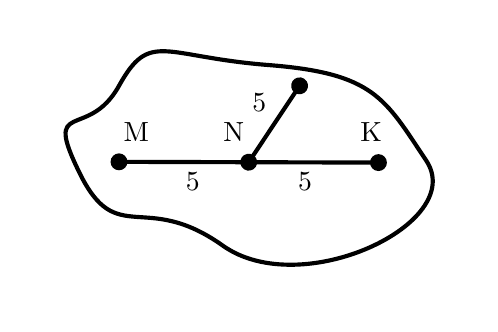
\begin{tikzpicture}[x=0.75pt,y=0.75pt,yscale=-1,xscale=1]
        \path (0,114); %set diagram left start at 0, and has height of 114
        
        %Shape: Polygon Curved [id:ds2132557395722765] 
        \draw  [line width=1.5]  (44,22.36) .. controls (59,-4.64) and (65,8.36) .. (116,12.36) .. controls (167,16.36) and (172,28.36) .. (192,58.36) .. controls (212,88.36) and (132,126.36) .. (94,99.36) .. controls (56,72.36) and (43,101.04) .. (25,64.36) .. controls (7,27.68) and (29,49.36) .. (44,22.36) -- cycle ;
        %Straight Lines [id:da8250050906940507] 
        \draw [line width=1.5]    (44,59) -- (169,59.36) ;
        \draw [shift={(169,59.36)}, rotate = 0.16] [color={rgb, 255:red, 0; green, 0; blue, 0 }  ][fill={rgb, 255:red, 0; green, 0; blue, 0 }  ][line width=1.5]      (0, 0) circle [x radius= 3.05, y radius= 3.05]   ;
        \draw [shift={(44,59)}, rotate = 0.16] [color={rgb, 255:red, 0; green, 0; blue, 0 }  ][fill={rgb, 255:red, 0; green, 0; blue, 0 }  ][line width=1.5]      (0, 0) circle [x radius= 3.05, y radius= 3.05]   ;
        %Straight Lines [id:da7350911076335458] 
        \draw [line width=1.5]    (131,22.36) -- (106.5,59.18) ;
        \draw [shift={(106.5,59.18)}, rotate = 123.64] [color={rgb, 255:red, 0; green, 0; blue, 0 }  ][fill={rgb, 255:red, 0; green, 0; blue, 0 }  ][line width=1.5]      (0, 0) circle [x radius= 3.05, y radius= 3.05]   ;
        \draw [shift={(131,22.36)}, rotate = 123.64] [color={rgb, 255:red, 0; green, 0; blue, 0 }  ][fill={rgb, 255:red, 0; green, 0; blue, 0 }  ][line width=1.5]      (0, 0) circle [x radius= 3.05, y radius= 3.05]   ;
        
        % Text Node
        \draw (45,38.8) node [anchor=north west][inner sep=0.75pt]   [align=left] {M};
        % Text Node
        \draw (93,38.8) node [anchor=north west][inner sep=0.75pt]   [align=left] {N};
        % Text Node
        \draw (159,38.8) node [anchor=north west][inner sep=0.75pt]   [align=left] {K};
        % Text Node
        \draw (75,62.8) node [anchor=north west][inner sep=0.75pt]   [align=left] {$\displaystyle 5$};
        % Text Node
        \draw (129,62.8) node [anchor=north west][inner sep=0.75pt]   [align=left] {$\displaystyle 5$};
        % Text Node
        \draw (107,24.8) node [anchor=north west][inner sep=0.75pt]   [align=left] {$\displaystyle 5$};
        \end{tikzpicture}        
\end{wrapfigure}
\[
    \begin{array}{c}
        B_8(M) = \{M, N\}\\
        B_6(N) = \{M, N, K\}
    \end{array}  
\]}
\vspace*{2cm}


\begin{definition}{(Normed space)}{}
    A (complex or real) vector space $V$ is called normed space if a function (`norm') $\nu: \ V \to \R$, denoted for $v \in V$ $||v||$, which satisfies the following axioms:
    \begin{enumerate*}
        \item Positive definite property:
        \[ 
            \nu\left(\vec{x}\right) > 0;
        \]
        \item Homogeneity \[
            \nu\left(\alpha \vec{x}\right) = |\alpha|\nu\left(\vec{x}\right);
        \]
        \item Triangle inequality $\forall x, y \in V$:
        \[ 
            \nu\left(\vec{x} + \vec{y}\right) \leq \nu\left(\vec{x}\right) + \nu\left(\vec{y}\right).
        \]
    \end{enumerate*}
\end{definition}
\Ex Euclidean norm:
        \[
            \left|\vec{x}\right|_2 = \sqrt{\sum\limits_{i=1}^n |x_i|^2}    
        \]

\begin{proposition}{}{}
    In a normed space $V$, the function $\rho\left(\vec{x},\vec{y}\right) = \nu\left(\vec{y} - \vec{x}\right)$ is a metric.
\end{proposition}
\begin{proof}
    For proving positive definition of function $\nu\left(\vec{x}, \vec{y}\right)$ we need a lemma:
    \begin{lemma}{}{}
        $\nu\left(\vec{0}\right) = 0$
    \end{lemma}
    \begin{proof}
        $\nu\left(0 \cdot \vec{0}\right) = 0 \cdot \nu\left(\vec{0}\right) = 0.$
    \end{proof}
    \begin{enumerate}
        \item Positive definition:
        \[ 
            \begin{array}{c}
                \displaystyle\rho\left(\vec{x}, \vec{y}\right) = \nu\left(\vec{y} - \vec{x}\right) > 0  \\
                \displaystyle \rho\left(\vec{x}, \vec{x}\right) = \nu\left(\vec{x} - \vec{x}\right) = \nu\left(\vec{0}\right) = 0 
            \end{array}
        \]
        \item Symmetric:
        \[
            \rho\left(\vec{x}, \vec{y}\right) = \nu\left(\vec{y} - \vec{x}\right) = |-1|\nu\left(\vec{x} - \vec{y}\right) = \nu\left(\vec{x} - \vec{y}\right) = \rho\left(\vec{y}, \vec{x}\right)
        \]
        \item Triangle inequality:
        \[
            \begin{array}{c}
                \rho\left(\vec{x}, \vec{y}\right) + \rho\left(\vec{y}, \vec{z}\right) = \nu\left(\vec{y} - \vec{x}\right) + \nu\left(\vec{z} - \vec{y}\right) \geq \\ \geq \nu\left(\vec{y} - \vec{x} + \vec{z} -\vec{y} \right) = \nu\left(\vec{z} - \vec{x}\right) = \rho\left(\vec{x}, \vec{z}\right)
            \end{array}
        \]
    \end{enumerate}
\end{proof}
\begin{note}{}{}
    Each normed space is a metric space.
\end{note}

\par
\Ex In the vector space $\R^n (\C^n)$ the following three norms are in common use:
    \begin{itemize}
        \item Manhattan norm (Taxicab norm):
        
    \end{itemize}

    {\begin{wrapfigure}{l}{0.4\textwidth}
        \scalebox{1.5}{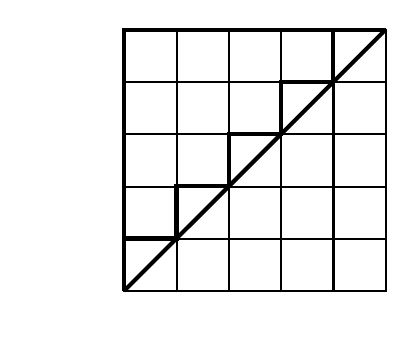
\begin{tikzpicture}[x=0.75pt,y=0.75pt,yscale=-1,xscale=1]
            \path (0,164); %set diagram left start at 0, and has height of 164
            
            %Shape: Grid [id:dp08042200947302103] 
            \draw  [draw opacity=0][line width=0.75]  (46.53,16.6) -- (172.55,16.6) -- (172.55,142.61) -- (46.53,142.61) -- cycle ; \draw  [line width=0.75]  (71.74,16.6) -- (71.74,142.61)(96.94,16.6) -- (96.94,142.61)(122.14,16.6) -- (122.14,142.61)(147.34,16.6) -- (147.34,142.61) ; \draw  [line width=0.75]  (46.53,41.8) -- (172.55,41.8)(46.53,67.01) -- (172.55,67.01)(46.53,92.21) -- (172.55,92.21)(46.53,117.41) -- (172.55,117.41) ; \draw  [line width=0.75]  (46.53,16.6) -- (172.55,16.6) -- (172.55,142.61) -- (46.53,142.61) -- cycle ;
            %Straight Lines [id:da6909809940649061] 
            \draw [line width=1.5]    (46.53,142.34) -- (172.43,16.6) ;
            %Straight Lines [id:da10608550876089407] 
            \draw [line width=1.5]    (46.53,142.34) -- (46.53,117.19) -- (71.71,117.19) -- (71.71,92.04) -- (96.89,92.04) -- (96.89,66.89) -- (122.07,66.89) -- (122.07,41.75) -- (147.25,41.75) -- (147.25,16.6) -- (172.43,16.6) ;
            %Straight Lines [id:da694529903122499] 
            \draw [line width=1.5]    (172.43,16.6) -- (46.53,16.6) -- (46.53,142.34) ;
            \end{tikzpicture}}            
    \end{wrapfigure}
    This is the norm of the following kind:
    \[
        ||x||_1 = \sum\limits_{i=1}^n |x_i|  
    \]
    \par 
    Let's prove that this function is a norm.
    \begin{enumerate}
        \item Positive definite property:
        Let $x \in \R^n$ or $x \in \C^n$. Obviously $||x||_1 \geq 0.$ Also $||x||_1 = 0$ iff $x = 0$.
        \item Homogeneity property:
        \useshortskip
        \[
            \forall c \in \R: \ ||c\cdot x||_1 = \sum\limits_{i=1}^n |c\cdot x_i| = |c| \cdot \sum\limits_{i=1}^n |x_i| = |c| \cdot ||x||_1 .
        \]
    \end{enumerate}}
    \begin{enumerate}
        \item[3.] Triangle inequality $\forall x, y \in \R^n$:
        \[
            \begin{array}{c}
                \displaystyle ||x+y||_1 = \sum\limits_{i=1}^n |x_i + y_i| \leq \sum\limits_{i=1}^n \left(|x_i| + |y_i|\right) = \\
                \displaystyle =              \sum\limits_{i=1}^n |x_i| + \sum\limits_{i=1}^n |y_i| = ||x||_1 + ||y||_1.     
            \end{array}
        \]
    \end{enumerate}
    \begin{itemize}
        \item Maximum norm (Infinity norm):
        \[
            ||x||_\infty = \max\limits_{1 \leq i \leq n} |x_i|.  
        \]
        \begin{enumerate}
            \item The function $||x||_\infty$ is positive since it is the maximum over a set of positive terms $|x_i|$.
            \item Homogeneity property:
            \[
                ||\alpha\cdot x ||_{\infty} = \max\limits_{1 \leq i \leq n} |\alpha\cdot x_i| = \max\limits_{1 \leq i \leq n} |\alpha| \cdot |x_i| = |\alpha| \cdot \max\limits_{1 \leq i \leq n} = |\alpha|\cdot ||x||_\infty. 
            \]
            \item Triangle inequality:
            \[
                ||x+y||_{\infty} = \max\limits_{1 \leq i \leq n} |x_i + y_i| \leq \max\limits_{1 \leq i \leq n} \left(|x_i| + |y_i|\right) \leq \max\limits_{1 \leq i \leq n} |x_i| + \max\limits_{1 \leq i \leq n} |y_i| = ||x||_\infty + ||y||_\infty.
            \]
        \end{enumerate}
    \end{itemize}

\Ex For the vector $x = \begin{bmatrix}
    1 \\
    2 \\ 
    -3 \\
    5
\end{bmatrix}$ we have:
\[
    ||x||_1 = 11; \ ||x||_2 = \sqrt{39}; \ ||x||_\infty = 5, 
\]
whereas for the vector $x = \begin{bmatrix}
    1+i \\
    2-3i\\
    4
\end{bmatrix}$,
\[
    ||x||_1 = \sqrt{2} + \sqrt{13} + 4; \ ||u||_2 = \sqrt{31}; \ ||u||_\infty = 4.  
\]

The notations $||\cdot ||_1, ||\cdot||_2$ and $||\cdot ||_\infty$ are justified because of the fact that all these norms are special cases of the general Minkovskiy $p-$norm:
\[
    ||x||_p = \sqrt[P]{\sum\limits_{i=1}^n |x_i|^p}, \ p\geq 1
\]
Similarly, in the vector space of real-valued continuous functions $\mathcal{C}[a,b]$, the following three norms are frequently used:
\[
    ||f||_1 = \int\limits_{a}^b |f(x)| dx; \ ||f||_2 = \sqrt{\int\limits_a^b f^2(x)dx}; \ ||f||_\infty = \max\limits_{x\in [a,b]} |f(x)|  
\]
And Minkovskiy norm:
\[
    ||f||_p = \sqrt[p]{\int\limits_{a}^b |f(x)|^p dx}  
\]
\par
For example, for $V = \mathcal{C}[0,1]$:

\[
    \begin{array}{c}
        \displaystyle ||f||_p = \sqrt[p]{\int\limits_{0}^1 |f(x)|^p dx}  \\
        \displaystyle ||f||_1 = \int\limits_{0}^1 |f(x)|^p dx\\
        \displaystyle ||f||_\infty = ||f||_0 = \max\limits_{x \in [0,1]} |f(x)|.
    \end{array}  
\]
\par 
Some weighted norms:

Let $V = \mathcal{C}[0,1]$; $\omega \geq 0$:

\[
    \begin{array}{c}
        \displaystyle ||f||_p^\omega = \left(\int\limits_0^1 |f(x)|^p \cdot \omega(x) dx\right)^\dfrac{1}{p} \\
        \displaystyle ||f||_\infty^\omega = ||f||_0^\omega = \max\limits_{x\in [0,1]} |f(x) \cdot \omega(x)|.
    \end{array}  
\]

\subsection*{Balls in normed space}
\begin{proposition}{}{}
    Let $V$ be a normed space
    \begin{itemize}
        \item All balls of the same radius $R$ are equal geometrically: a parallel translation of $B_R(\vec{x})$ by a vector $\vec{v} = \vec{y} - \vec{x}$ makes $B_R(\vec{y})$.
        \item For any two balls: $B = B_r(0)$ and $B' = B_R(0)$, there is a homotety $x \longmapsto \lambda \vec{x}$, which transfers $B$ onto $B'$, where $\lambda = \dfrac{R}{r}$. Also $B_1^p(0) = $ unit ball for $0$-norm.
    \end{itemize}
\end{proposition}
\begin{proof}
{\begin{wrapfigure}{r}{0.4\textwidth}
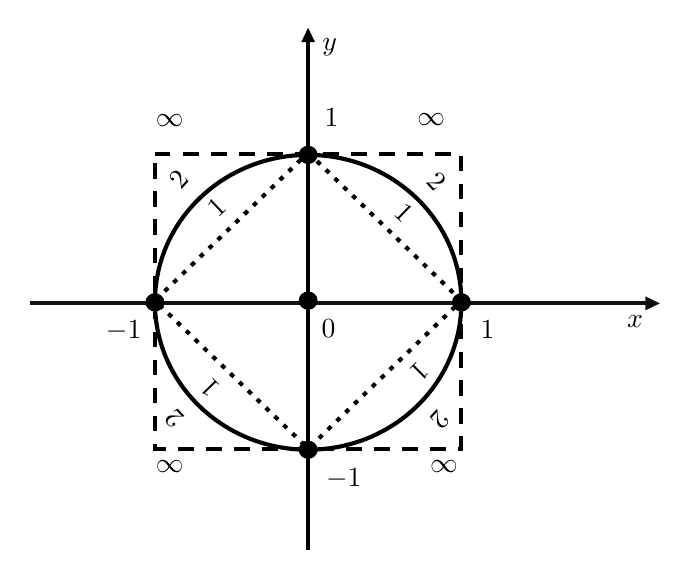
\begin{tikzpicture}[x=0.75pt,y=0.75pt,yscale=-1,xscale=1]
    %uncomment if require: \path (0,300); %set diagram left start at 0, and has height of 300
    
    %Straight Lines [id:da8306888936977477] 
    \draw [line width=1.5]    (175.02,17) -- (175.02,264.39) ;
    \draw [shift={(175.02,13)}, rotate = 90] [fill={rgb, 255:red, 0; green, 0; blue, 0 }  ][line width=0.08]  [draw opacity=0] (6.97,-3.35) -- (0,0) -- (6.97,3.35) -- cycle    ;
    %Straight Lines [id:da5110121506356493] 
    \draw [color={rgb, 255:red, 16; green, 16; blue, 16 }  ,draw opacity=1 ][fill={rgb, 255:red, 4; green, 4; blue, 4 }  ,fill opacity=1 ][line width=1.5]    (340.5,145.77) -- (40.89,145.77) ;
    \draw [shift={(344.5,145.77)}, rotate = 180] [fill={rgb, 255:red, 16; green, 16; blue, 16 }  ,fill opacity=1 ][line width=0.08]  [draw opacity=0] (6.97,-3.35) -- (0,0) -- (6.97,3.35) -- cycle    ;
    %Shape: Ellipse [id:dp06424647272445538] 
    \draw  [line width=1.5]  (101.19,145.27) .. controls (101.19,106.04) and (134.25,74.24) .. (175.02,74.24) .. controls (215.8,74.24) and (248.85,106.04) .. (248.85,145.27) .. controls (248.85,184.49) and (215.8,216.29) .. (175.02,216.29) .. controls (134.25,216.29) and (101.19,184.49) .. (101.19,145.27) -- cycle ;
    %Shape: Rectangle [id:dp9119970932820067] 
    \draw  [dash pattern={on 5.63pt off 4.5pt}][line width=1.5]  (101.19,73.71) -- (248.85,73.71) -- (248.85,215.76) -- (101.19,215.76) -- cycle ;
    %Shape: Diamond [id:dp4333715282427959] 
    \draw  [dash pattern={on 1.69pt off 2.76pt}][line width=1.5]  (175.02,73.14) -- (248.85,144.45) -- (175.02,215.76) -- (101.19,144.45) -- cycle ;
    %Shape: Ellipse [id:dp8226317539510353] 
    \draw  [fill={rgb, 255:red, 0; green, 0; blue, 0 }  ,fill opacity=1 ] (170.74,144.45) .. controls (170.74,142.18) and (172.66,140.33) .. (175.02,140.33) .. controls (177.39,140.33) and (179.31,142.18) .. (179.31,144.45) .. controls (179.31,146.73) and (177.39,148.58) .. (175.02,148.58) .. controls (172.66,148.58) and (170.74,146.73) .. (170.74,144.45) -- cycle ;
    %Shape: Ellipse [id:dp08502683026718438] 
    \draw  [fill={rgb, 255:red, 0; green, 0; blue, 0 }  ,fill opacity=1 ] (244.57,145.27) .. controls (244.57,142.99) and (246.49,141.14) .. (248.85,141.14) .. controls (251.22,141.14) and (253.14,142.99) .. (253.14,145.27) .. controls (253.14,147.54) and (251.22,149.39) .. (248.85,149.39) .. controls (246.49,149.39) and (244.57,147.54) .. (244.57,145.27) -- cycle ;
    %Shape: Ellipse [id:dp4574361474994544] 
    \draw  [fill={rgb, 255:red, 0; green, 0; blue, 0 }  ,fill opacity=1 ] (96.91,145.27) .. controls (96.91,142.99) and (98.82,141.14) .. (101.19,141.14) .. controls (103.56,141.14) and (105.48,142.99) .. (105.48,145.27) .. controls (105.48,147.54) and (103.56,149.39) .. (101.19,149.39) .. controls (98.82,149.39) and (96.91,147.54) .. (96.91,145.27) -- cycle ;
    %Shape: Ellipse [id:dp9128016551294487] 
    \draw  [fill={rgb, 255:red, 0; green, 0; blue, 0 }  ,fill opacity=1 ] (170.74,74.24) .. controls (170.74,71.96) and (172.66,70.11) .. (175.02,70.11) .. controls (177.39,70.11) and (179.31,71.96) .. (179.31,74.24) .. controls (179.31,76.51) and (177.39,78.36) .. (175.02,78.36) .. controls (172.66,78.36) and (170.74,76.51) .. (170.74,74.24) -- cycle ;
    %Shape: Ellipse [id:dp34957400582859055] 
    \draw  [fill={rgb, 255:red, 0; green, 0; blue, 0 }  ,fill opacity=1 ] (170.74,216.29) .. controls (170.74,214.02) and (172.66,212.17) .. (175.02,212.17) .. controls (177.39,212.17) and (179.31,214.02) .. (179.31,216.29) .. controls (179.31,218.57) and (177.39,220.42) .. (175.02,220.42) .. controls (172.66,220.42) and (170.74,218.57) .. (170.74,216.29) -- cycle ;
    
    % Text Node
    \draw (180.27,152.42) node [anchor=north west][inner sep=0.75pt]   [align=left] {$\displaystyle 0$};
    % Text Node
    \draw (76.36,152.67) node [anchor=north west][inner sep=0.75pt]   [align=left] {$\displaystyle -1$};
    % Text Node
    \draw (256.83,152.67) node [anchor=north west][inner sep=0.75pt]   [align=left] {$\displaystyle 1$};
    % Text Node
    \draw (182.38,223.97) node [anchor=north west][inner sep=0.75pt]   [align=left] {$\displaystyle -1$};
    % Text Node
    \draw (181.75,50.91) node [anchor=north west][inner sep=0.75pt]   [align=left] {$\displaystyle 1$};
    % Text Node
    \draw (226.43,53) node [anchor=north west][inner sep=0.75pt]   [align=left] {$\displaystyle \infty $};
    % Text Node
    \draw (232.5,220.22) node [anchor=north west][inner sep=0.75pt]   [align=left] {$\displaystyle \infty $};
    % Text Node
    \draw (100.43,220.22) node [anchor=north west][inner sep=0.75pt]   [align=left] {$\displaystyle \infty $};
    % Text Node
    \draw (100.43,53.73) node [anchor=north west][inner sep=0.75pt]   [align=left] {$\displaystyle \infty $};
    % Text Node
    \draw (221.69,94.87) node [anchor=north west][inner sep=0.75pt]  [rotate=-43.96] [align=left] {$\displaystyle 1$};
    % Text Node
    \draw (123.83,98.41) node [anchor=north west][inner sep=0.75pt]  [rotate=-316.59] [align=left] {$\displaystyle 1$};
    % Text Node
    \draw (126.89,193.78) node [anchor=north west][inner sep=0.75pt]  [rotate=-225.71] [align=left] {$\displaystyle 1$};
    % Text Node
    \draw (235.69,179.51) node [anchor=north west][inner sep=0.75pt]  [rotate=-135.19] [align=left] {$\displaystyle 1$};
    % Text Node
    \draw (105.42,86.05) node [anchor=north west][inner sep=0.75pt]  [rotate=-311.39] [align=left] {$\displaystyle 2$};
    % Text Node
    \draw (237.7,79.66) node [anchor=north west][inner sep=0.75pt]  [rotate=-47.02] [align=left] {$\displaystyle 2$};
    % Text Node
    \draw (245.64,202.2) node [anchor=north west][inner sep=0.75pt]  [rotate=-133.09] [align=left] {$\displaystyle 2$};
    % Text Node
    \draw (109.66,208.34) node [anchor=north west][inner sep=0.75pt]  [rotate=-226.72] [align=left] {$\displaystyle 2$};
    % Text Node
    \draw (327.49,150.48) node [anchor=north west][inner sep=0.75pt]   [align=left] {$\displaystyle x$};
    % Text Node
    \draw (180.61,16.85) node [anchor=north west][inner sep=0.75pt]   [align=left] {$\displaystyle y$};
    
    
    \end{tikzpicture}
\end{wrapfigure}   
    \begin{enumerate}
        \item 
        \[
            \begin{array}{c}
               \displaystyle B_R(\vec{x}) + V = \left\{\vec{a}\ | \ \nu\left(\vec{a} - \vec{x}\right) \leq R\right\} + \left(\vec{y} - \vec{x}\right) =  \\ 
               \displaystyle = \left\{\vec{a} + \vec{y} - \vec{x}\ | \ \nu\left(\vec{a} - \vec{x}\right) \leq R\right\} = \left\{\vec{b}\ | \ \nu\left(\vec{b} - \vec{y}\right) \leq R \right\} = \\
               \displaystyle = B_R(\vec{y}), \text{ where: } \vec{a} + \vec{y} - \vec{x} = \vec{b}; \ \vec{a} = \vec{b} - \vec{y} + \vec{x}.
            \end{array}
        \]
        \item $\dfrac{R}{r} \cdot \vec{a} = \vec{b}$; $\vec{a} = \dfrac{r}{R} \cdot \vec{b}$.
        \[
            \begin{array}{c}
                \displaystyle \lambda \cdot B = \dfrac{R}{r}\cdot \left\{\vec{a}\ | \ \nu\left(\vec{a}\right) \leq r\right\} = \left\{\dfrac{R}{r} \cdot \vec{a} \ | \ \nu\left(\vec{a}\right) \leq r\right\} = \\
                \displaystyle = \left\{\vec{b}\ | \ \nu\left(\dfrac{r}{R} \cdot \vec{b}\right) \leq r\right\} = \left\{\vec{b}\ | \ \dfrac{r}{R} \cdot \nu \left(\vec{b}\right) \leq r\right\} = \\
                \displaystyle = \left\{\vec{b}\ | \ \nu\left(\vec{b}\right) \leq \dfrac{r\cdot R}{r}\right\} = \left\{\vec{b} \ | \ \nu\left(\vec{b}\right) \leq R\right\} = B'.
            \end{array}  
        \]
    \end{enumerate} }
\end{proof}